%% This template can be used to write a paper for
%% Computer Physics Communications using LaTeX.
%% For authors who want to write a computer program description,
%% an example Program Summary is included that only has to be
%% completed and which will give the correct layout in the
%% preprint and the journal.
%% The `elsarticle' style is used and more information on this style
%% can be found at 
%% http://www.elsevier.com/wps/find/authorsview.authors/elsarticle.
%%
%%
\documentclass[preprint,12pt]{elsarticle}

%% Use the option review to obtain double line spacing
%% \documentclass[preprint,review,12pt]{elsarticle}

%% Use the options 1p,twocolumn; 3p; 3p,twocolumn; 5p; or 5p,twocolumn
%% for a journal layout:
%% \documentclass[final,1p,times]{elsarticle}
%% \documentclass[final,1p,times,twocolumn]{elsarticle}
%% \documentclass[final,3p,times]{elsarticle}
%% \documentclass[final,3p,times,twocolumn]{elsarticle}
%% \documentclass[final,5p,times]{elsarticle}
%% \documentclass[final,5p,times,twocolumn]{elsarticle}

%% if you use PostScript figures in your article
%% use the graphics package for simple commands
%% \usepackage{graphics}
%% or use the graphicx package for more complicated commands
\usepackage{graphicx}
%% or use the epsfig package if you prefer to use the old commands
%% \usepackage{epsfig}

%% The amssymb package provides various useful mathematical symbols
\usepackage{amssymb}
%% The amsthm package provides extended theorem environments
%% \usepackage{amsthm}

%% Additional needed packages.
\usepackage{amsmath}
\usepackage{verbatim}
\usepackage{color}

%% The lineno packages adds line numbers. Start line numbering with
%% \begin{linenumbers}, end it with \end{linenumbers}. Or switch it on
%% for the whole article with \linenumbers after \end{frontmatter}.
\usepackage{lineno}
\usepackage{hyperref}

%% natbib.sty is loaded by default. However, natbib options can be
%% provided with \biboptions{...} command. Following options are
%% valid:

%%   round  -  round parentheses are used (default)
%%   square -  square brackets are used   [option]
%%   curly  -  curly braces are used      {option}
%%   angle  -  angle brackets are used    <option>
%%   semicolon  -  multiple citations separated by semi-colon
%%   colon  - same as semicolon, an earlier confusion
%%   comma  -  separated by comma
%%   numbers-  selects numerical citations
%%   super  -  numerical citations as superscripts
%%   sort   -  sorts multiple citations according to order in ref. list
%%   sort&compress   -  like sort, but also compresses numerical citations
%%   compress - compresses without sorting
%%
%% \biboptions{comma,round}

% \biboptions{}

\newcommand{\pdv}[2]{\frac{\partial{#1}}{\partial{#2}}}
\newcommand{\fp}[2]{\pdv{#1}{#2}}
\newcommand{\pdwc}[3]{\left(\fp{#1}{#2}\right)_{#3}}
%\newcommand{\ppdv}[3]{\displaystyle \frac{\partial^2 #1}{\partial #2\partial #3}}
\newcommand{\ppdv}[3]{\frac{\partial^2 #1}{\partial #2\partial #3}}
\newcommand{\oover}[1]{\ensuremath{\frac{1}{#1}}}

\newcommand{\vect}[1]{\boldsymbol{#1}}
\newcommand{\matr}[1]{\mathbf{#1}}
\newcommand{\dI}{\text{d}}
\newcommand{\odv}[2]{\frac{\dI #1}{\dI #2}}
\newcommand{\ddv}[2]{\odv{#1}{#2}}
\newcommand{\christ}[3]{\genfrac{\{}{\}}{0pt}{}{#1}{#2 #3}}
%\newcommand{\christ}[3]{\Gamma^{#1}_{#2 #3}}
%\newcommand{\ddv}[2]{\frac{\Delta #1}{\Delta #2}}
\newcommand{\collpdv}[2]{\pdv{#1}{#2}\Big|_{coll}}
\newcommand{\mfp}{\lambda}
\newcommand{\tmfp}{\tilde{\lambda}}
\newcommand{\mfpe}{\lambda_e}
\newcommand{\mfpei}{\lambda_{ei}}
\newcommand{\Zbar}{\bar{Z}}
\newcommand{\nue}{\nu_{e}}
\newcommand{\nuei}{\nu_{ei}}
\newcommand{\nutot}{\nu_{t}}
\newcommand{\vmag}{v}
\newcommand{\vth}{v_{th}}
\newcommand{\vn}{\vect{n}}
\newcommand{\E}{\vect{E}}
\newcommand{\B}{\vect{B}}
\newcommand{\tE}{\vect{\tilde{E}}}
\newcommand{\tEz}{\tilde{E}_z}
\newcommand{\tB}{\vect{\tilde{B}}}
\newcommand{\qe}{q_e}
\newcommand{\me}{m_e}
\newcommand{\kB}{k_B}
\newcommand{\crs}{\sigma}
\newcommand{\fM}{f_M}
\newcommand{\tfM}{\tilde{f}_M}
\newcommand{\tvfM}{\vect{\tilde{f}_M}}
\newcommand{\daf}{\delta f}
\newcommand{\fzero}{f_0}
\newcommand{\dafzero}{\delta f_0}
\newcommand{\vfzero}{\vect{f_0}}
\newcommand{\davfzero}{\vect{\delta f_0}}
\newcommand{\fone}{\vect{f_1}}
\newcommand{\fonez}{f_{1_z}}
\newcommand{\SM}{\vect{S}_M}
\newcommand{\MI}{\matr{I}}
\newcommand{\MA}{\matr{A}}
\newcommand{\intO}{\int_{\Omega}}
\newcommand{\intv}{\int_{\vmag}}
\newcommand{\IM}{\boldsymbol{\mathcal{M}}}
\newcommand{\ID}{\boldsymbol{\mathcal{D}}}
\newcommand{\IV}{\boldsymbol{\mathcal{V}}}
\newcommand{\IB}{\boldsymbol{\mathcal{B}}}
\newcommand{\anisomega}{\fone/\fzero}
\newcommand{\acl}{\vect{M}_{\left(\anisomega\right)}}

\newcommand{\Wzero}{\psi}
\newcommand{\Wone}{\matr{w}}
\newcommand{\Wcurl}{\vect{W_c}}
\newcommand{\Wdiv}{\vect{W_d}}



\newcommand{\figref}[1]{FIG.~\ref{#1}}
\newcommand{\refeq}[1]{(\ref{#1})}
\newcommand{\secref}[1]{Sec.~\ref{#1}}


%% This list environment is used for the references in the
%% Program Summary
%%
\newcounter{bla}
\newenvironment{refnummer}{%
\list{[\arabic{bla}]}%
{\usecounter{bla}%
 \setlength{\itemindent}{0pt}%
 \setlength{\topsep}{0pt}%
 \setlength{\itemsep}{0pt}%
 \setlength{\labelsep}{2pt}%
 \setlength{\listparindent}{0pt}%
 \settowidth{\labelwidth}{[9]}%
 \setlength{\leftmargin}{\labelwidth}%
 \addtolength{\leftmargin}{\labelsep}%
 \setlength{\rightmargin}{0pt}}}
 {\endlist}

\journal{Computer Physics Communications}

\begin{document}

\begin{frontmatter}

%% Title, authors and addresses

%% use the tnoteref command within \title for footnotes;
%% use the tnotetext command for the associated footnote;
%% use the fnref command within \author or \address for footnotes;
%% use the fntext command for the associated footnote;
%% use the corref command within \author for corresponding author footnotes;
%% use the cortext command for the associated footnote;
%% use the ead command for the email address,
%% and the form \ead[url] for the home page:
%%
%% \title{Title\tnoteref{label1}}
%% \tnotetext[label1]{}
%% \author{Name\corref{cor1}\fnref{label2}}
%% \ead{email address}
%% \ead[url]{home page}
%% \fntext[label2]{}
%% \cortext[cor1]{}
%% \address{Address\fnref{label3}}
%% \fntext[label3]{}

\title{An~efficient kinetic modeling in hydrodynamics using the AWBS transport equation}

%% use optional labels to link authors explicitly to addresses:
%% \author[label1,label2]{<author name>}
%% \address[label1]{<address>}
%% \address[label2]{<address>}

%\author[a]{M. Holec\corref{author}}
\author[a,b]{Authors}
%\author[b]{Third Author}

\cortext[author] {Corresponding author.\\\textit{E-mail address:} milan.holec@u-bordeaux.fr}
\address[a]{Centre Lasers Intenses et Applications, Universite de Bordeaux-CNRS-CEA, UMR 5107, F-33405 Talence, France}
%\address[b]{Second Address}

\begin{abstract}
The~AWBS Boltzmann transport equation for electrons equipped with 
a~simplified e-e collision operator~\cite{AWBS_PRL1986}
provides an~efficient, yet physically 
relevant, kinetic extension compared the~classical 
Spitzer-Harm heat flux (SH)
based on local approximation and flux-limiting.
This classical approach is widely used in plasma
kinetics models coupled to hydrodynamics. 
Even though SH reflects the~electron-electron collision effect, 
the essential physical properties
%, e.g. non-locality due to appropriate electron 
%distribution function, 
of the~electron transport cannot be modeled with 
an~explicitly local model. A~simple form of the~AWBS model opens a~way 
to couple kinetics to hydrodynamic codes while describing the~important 
physics correctly. Since the~electron-electron collision effect becomes 
especially important in the~case of low ion potential, we take a~special in 
the~case of low Z plasmas.
\end{abstract}

\begin{keyword}
%% keywords here, in the form: keyword \sep keyword
kinetics; hydrodynamics; nonlocal electron transport; laser-heated plasmas.

\end{keyword}

\end{frontmatter}

%%
%% Start line numbering here if you want
%%
 \linenumbers

\tableofcontents
%% main text
%\section{}
%\label{}
%---------------------------------------------------------------------
%---------------------------------------------------------------------

\section{AWBS-P1 modeling of laser heated plasmas}\label{sec:OOE_AWBSP1}
\subsection{Model equations}
The~AWBS electron transport equation reads
\begin{multline}
  \vmag\vn\cdot\nabla f + \tE\cdot\vn \pdv{f}{\vmag} 
  + \frac{\tE\cdot\vect{e}_\phi 
  - \vmag\tB\cdot\vect{e}_\theta}{\vmag}\pdv{f}{\phi}
  =
  \vmag \nue \pdv{}{\vmag}\left(f - f_M\right) 
  + (\nuei + \nue) (\fzero - f) ,
  \nonumber \label{eq:AWBS_model}
\end{multline}
where $\nue$ is the~electron-electron collision frequency, 
$\nuei$ is the~electron-ion collision frequency, and $\nuei = \Zbar \nue$.

In order to eliminate the~dimensions of the~above transport problem 
the~first-two-moment model based on approximation 
\begin{equation}
  f = \frac{\fzero}{4\pi} + \frac{3}{4\pi}\vn\cdot\fone , 
  \nonumber \label{eq:OOE_P1approximation}
\end{equation}
can be adopted and reads
\begin{eqnarray}
  \nue\vmag\pdv{}{\vmag}\left(\fzero - \tfM \right) &=&
  \vmag\nabla\cdot\fone + \tE\cdot
  \pdv{\fone}{\vmag} + \frac{2}{\vmag}\tE\cdot\fone , 
  \nonumber \label{eq:OOE_P1f0}\\
  \nue\vmag\pdv{}{\vmag}\fone - \nutot\fone &=& 
  \vmag\nabla\cdot\left(\MA\fzero\right) + 
  \tE\cdot\pdv{\left(\MA\fzero\right)}{\vmag} + \tB\times\fone ,
  \nonumber \label{eq:OOE_P1f1}
\end{eqnarray}
where $\tfM = 4\pi \fM$ and the~closure matrix takes the~form
\begin{equation}
  \MA = \frac{1}{3}\MI .
  \nonumber \label{eq:OOE_P1closure}
\end{equation}

Since in the~laser heated plasmas the~Knudsen number 
Kn$ = \frac{\vth}{\nu_t(\vth) L} \in (0, 1)$, i.e. the~collisionality in 
the~kinetics of electrons plays always an~important effect for thermal-like 
particles, the~electron distribution 
function can be treated as out-of-equilibrium approximation 
\begin{equation}
  f = \fM + \daf ,
  \label{eq:OOE_outofeq}
\end{equation}  
where the~consequent AWBS model reads
\begin{multline}
  \vmag\vn\cdot\nabla (\fM + \daf) + \tE\cdot\vn \pdv{\fM}{\vmag} 
  + \tE\cdot\vn \pdv{\daf}{\vmag} 
  + \frac{\tE\cdot\vect{e}_\phi 
  - \vmag\tB\cdot\vect{e}_\theta}{\vmag}\pdv{\daf}{\phi}
  = \\
  \vmag \nue \pdv{\daf}{\vmag} 
  + (\nuei + \nue) (\fzero - \fM - \daf) ,
  \label{eq:OOE_AWBS_model}
\end{multline}
or its P1 approximation equivalent
\begin{equation}
  f = \frac{4\pi \fM + \dafzero}{4\pi} + \frac{3}{4\pi}\vn\cdot\fone .
  \label{eq:OOE_P1outofeq}
\end{equation}
where the~moment model reads
\begin{eqnarray}
  \nue\vmag\pdv{\dafzero}{\vmag} &=&
  \vmag\nabla\cdot\fone + \tE\cdot
  \pdv{\fone}{\vmag} + \frac{2}{\vmag}\tE\cdot\fone , 
  \label{eq:OOE_P1f0}\\
  \nue\vmag\pdv{\fone}{\vmag} - \nutot\fone &=& 
  \frac{\vmag}{3}\nabla\dafzero + 
  \frac{\tE}{3}\pdv{\dafzero}{\vmag} + \tB\times\fone 
  \nonumber \\
  & & + \frac{\vmag}{3}\nabla\tfM + \frac{\tE}{3}\pdv{\tfM}{\vmag} .
  \label{eq:OOE_P1f1}
\end{eqnarray}

\subsection{A~consistent treatment of $\tE$ field}
\label{sec:OOE_E_treatment}
\begin{equation}
  \vect{q}_c(\vect{x}) = \intv
  \vmag\fone(\vect{x}) \vmag^2\, \dI\vmag , \nonumber 
\end{equation}
from \eqref{eq:OOE_P1f1}
\begin{equation}
  %\frac{\vect{j}}{\qe} = 
  \vect{q}_c =
  \intv \left(\frac{\nue\vmag^2}{\nutot}\pdv{\fone}{\vmag}
  - \frac{\vmag^2}{3\nutot}\nabla\left(\tfM + \dafzero\right) - 
  \frac{\vmag}{3\nutot}\pdv{\left(\tfM + \dafzero\right)}{\vmag}\tE
  \right) \vmag^2\, \dI\vmag ,
  \label{eq:OOE_P1current}
\end{equation}

\begin{eqnarray}
  a_0(\vect{x}) &=& \intv\frac{\vmag}{3 \nutot} \pdv{\left(\tfM + \dafzero\right)}{\vmag}(\vect{x})
  \vmag^2\, \dI\vmag , \nonumber \\
  \vect{b}_{0}(\vect{x}) &=& \intv\left(  
  \frac{\vmag^2}{3 \nutot}\nabla\left(\tfM(\vect{x}) + \dafzero(\vect{x})\right)
  - \frac{\nue\vmag^2}{\nutot}\pdv{\fone}{\vmag}(\vect{x})
  \right)\vmag^2\, \dI\vmag , \nonumber 
\end{eqnarray}
%Alors, treat $a_0, \vect{b}_{0}, \vect{b}_1$ as grid functions, 
%where it is obvious to express 
%$\pdv{a_0}{\vmag}, \pdv{\vect{b}_{0}}{\vmag}, \pdv{\vect{b}_1}{\vmag}$ in 
%ImplicitSolve().

\begin{equation}
  \vect{q}_c(\vect{x}) 
  = -\vect{b}_{0}(\vect{x}) 
  - a_{0}(\vect{x})\tE(\vect{x}) ,
  \nonumber \label{eq:OOE_HOFcurrent}
\end{equation}

%\begin{equation}
%  \tE(\vect{x}) = -\frac{\vect{b}_{0}(\vect{x})}{a_{0}(\vect{x})} 
%  - \frac{\vect{q}_c(\vect{x})}{a_{0}(\vect{x})}
%   + \frac{\vect{b}_{1}(\vect{x})}{a_{0}(\vect{x})}\times\tB(\vect{x}) ,
%  \nonumber \label{eq:OOE_HOFcurrent}
%\end{equation}

\begin{equation}
  \tE(\vect{x}) = -\frac{\vect{b}_{0}(\vect{x})}{a_{0}(\vect{x})} .
  \label{eq:OOE_E_j0}
\end{equation}

\subsection{AWBS model analysis}
\label{sec:OOE_AWBS_model_analysis}
\begin{multline}
  \left(\vmag \nue - \tE\cdot\vn\right)\pdv{\daf}{\vmag} 
  %+ \frac{\tE\cdot\vect{e}_\phi 
  %- \vmag\tB\cdot\vect{e}_\theta}{\vmag}\pdv{f}{\phi}
  =
  \vmag\vn\cdot\nabla (\fM + \daf) + \tE\cdot\vn\pdv{\fM}{\vmag} 
  + (\nuei + \nue) (\fM + \daf - \fzero) ,
  \label{eq:OOE_AWBS_model_analysis}
\end{multline}

\begin{eqnarray}
  \pdv{\dafzero}{\vmag} &=&
  \frac{1}{\nue\vmag}\left(\vmag\nabla\cdot\fone + \tE\cdot
  \pdv{\fone}{\vmag}\right) , 
  \nonumber\\
  \nue\vmag\pdv{\fone}{\vmag} - \nutot\fone &=& 
  \frac{\vmag}{3}\nabla\dafzero + 
  \frac{\tE}{3}\pdv{\dafzero}{\vmag}
  + \frac{\vmag}{3}\nabla\tfM + \frac{\tE}{3}\pdv{\tfM}{\vmag} ,
  \nonumber
\end{eqnarray}

\begin{equation}
  \left(\nue\vmag\MI - \frac{\tE\tE}{3 \nue\vmag}\right)\cdot
  \pdv{\fone}{\vmag} = 
  \frac{\vmag}{3}\nabla\dafzero + \frac{\tE}{3 \nue}\nabla\cdot\fone
  + \frac{\vmag}{3}\nabla\tfM + \frac{\tE}{3}\pdv{\tfM}{\vmag} 
  + \nutot\fone,
  \nonumber \label{eq:OOE_P1AWBS_model_analysis}
\end{equation}

\begin{equation}
  \left(\nue\vmag - \frac{\tEz^2}{3 \nue\vmag}\right)
  \pdv{\fonez}{\vmag} = 
  \frac{\vmag}{3}\pdv{\dafzero}{z} + \frac{\tEz}{3 \nue}\pdv{\fonez}{z}
  + \frac{\vmag}{3}\pdv{\tfM}{z} + \frac{\tEz}{3}\pdv{\tfM}{\vmag} 
  + \nutot\fonez .
  \label{eq:OOE_P1AWBS_model_1Danalysis}
\end{equation}

\begin{comment} % Implicit fully-discrete scheme
\subsection{Implicit fully-discrete scheme}
\label{sec:OOE_impl_fullydiscrete_scheme}
The moment P1 model \eqref{eq:OOE_P1f0}, \eqref{eq:OOE_P1f1} can be written 
in a~semi-discrete form
\begin{eqnarray}
  \IM^0_{(\nue)} \cdot \pdv{\davfzero}{\vmag}  
  &=& 
  \left(\ID^T_{\left(\MI\right)}
  + \frac{2}{\vmag^2}\IV^T_{\left(\tE\right)}\right) \cdot \fone
  + \frac{1}{\vmag}\IV^T_{\left(\tE\right)} \cdot 
  \pdv{\fone}{\vmag} ,  
  \nonumber \label{eq:OOE_semiM1hosf0} \\
  \IM^1_{(\nue)} \cdot \pdv{\fone}{\vmag}  
  &=& 
  - \ID_{\left(\MA\right)}\cdot\davfzero
  + \frac{1}{\vmag}\IV_{\left(\MA \cdot \tE\right)} \cdot
  \pdv{\davfzero}{\vmag}
  + \frac{1}{\vmag}\left(
  \IM^1_{\left( \nutot \right)} + \IB_{\left( \tB \right)}  
  \right) \cdot \fone
  \nonumber\\
  & & - \ID_{\left(\MA\right)}\cdot \tvfM
  + \frac{1}{\vmag}\IV_{\left(\MA \cdot \tE\right)} \cdot
  \pdv{\tvfM}{\vmag} .
  \label{eq:OOE_semiM1hosf1}
\end{eqnarray}
It is convenient to define
\begin{equation}
  \matr{DIVE} = \ID^T_{\left(\MI\right)} 
  + \frac{2}{\vmag^2}\IV^T_{\left(\tE\right)}.
  \nonumber
\end{equation}
The next step goes towards implicit Runge-Kutta method (DIRK).
Then, a~very effective inversion in the~L2 space can be formally performed
\begin{equation}
  \pdv{\davfzero}{\vmag}  
  = \frac{1}{\vmag}
  \IM^{0^{-1}}_{(\nue)} \cdot \IV^T_{\left(\tE\right)} \cdot 
  \pdv{\fone}{\vmag} 
  + \IM^{0^{-1}}_{(\nue)} \cdot \matr{DIVE}\cdot  
  \left(\fone^n 
  + \Delta\vmag\pdv{\fone}{\vmag}\right) .
  \label{eq:OOE_fullP1hosf0}
\end{equation}
The~first moment equation in the DIRK framework reads
\begin{multline}
  \IM^1_{(\nue)} \cdot \pdv{\fone}{\vmag}  
  = \frac{1}{\vmag}\IV_{\left(\MA \cdot \tE\right)} \cdot
  \pdv{\davfzero}{\vmag}
  - \ID_{\left(\MA\right)}\cdot \left(\tvfM^n + \davfzero^n 
  + \Delta\vmag\pdv{\davfzero}{\vmag}\right)\\ 
  + \frac{1}{\vmag}\left(\IB_{\left( \tB \right)} 
  + \IM^1_{\left( \nutot \right)}\right) 
  \cdot \left(\fone^n 
  + \Delta\vmag\pdv{\fone}{\vmag}\right)
  + \frac{1}{\vmag}\IV_{\left(\MA \cdot \tE\right)} \cdot
  \pdv{\tvfM^n}{\vmag} .
  \label{eq:OOE_semiM1hosf1}
\end{multline}
Finally, one can eliminate $\pdv{\davfzero}{\vmag}$, 
which leads to the~final form
\begin{multline}
  \IM^1_{(\nue)} \cdot \pdv{\fone}{\vmag}  
  = 
  \left(\frac{1}{\vmag}\IV_{\left(\MA \cdot \tE\right)}
  - \Delta\vmag \ID_{\left(\MA\right)} \right) \cdot
  \IM^{0^{-1}}_{(\nue)} \cdot 
  \left(\frac{1}{\vmag} \IV^T_{\left(\tE\right)} 
  + \Delta\vmag \matr{DIVE}
  \right)
  \cdot \pdv{\fone}{\vmag}
  \\
  +\frac{\Delta\vmag}{\vmag}\left(\IB_{\left( \tB \right)} 
  + \IM^1_{\left( \nutot \right)}\right) 
  \cdot \pdv{\fone}{\vmag} + 
  \frac{1}{\vmag}\left(\IB_{\left( \tB \right)} 
  + \IM^1_{\left( \nutot \right)}\right) 
  \cdot \fone^n
  + \frac{1}{\vmag}\IV_{\left(\MA \cdot \tE\right)} \cdot
  \pdv{\tvfM^n}{\vmag}
  \\ 
  +\left(\frac{1}{\vmag}\IV_{\left(\MA \cdot \tE\right)}
  - \Delta\vmag \ID_{\left(\MA\right)} \right) \cdot
  \IM^{0^{-1}}_{(\nue)} \cdot \matr{DIVE}\cdot\fone^n 
  - \ID_{\left(\MA\right)}\cdot\left(\tvfM^n + \davfzero^n\right),
  \label{eq:OOE_fullP1hosf1}
\end{multline}
where the~only unknown is $\pdv{\fone}{\vmag}$. Once \eqref{eq:OOE_fullP1hosf1}
is solved the~completion of the~solution 
$[\pdv{\davfzero}{\vmag}, \pdv{\fone}{\vmag}]$ is achieved by evaluating 
\eqref{eq:OOE_fullP1hosf0}.
\cite{Dobrev_Kolev_Rieben-High-order_curvilinear_finite_element_methods_for_Lagrangian_hydrodynamics}
\end{comment} % Implicit fully-discrete scheme

\section{Simulation results}\label{sec:results}
Two cases:
\begin{itemize}
  \item constant $n_e = 5\times10^{20}$ [1/cm$^3$], constant $\Zbar = 4$, 
  $T_e$ temperature profile taken from IMPACT simulation at 12 ps, see Figure 1
  %\figref{fig:Philippe_VFP_12ps}
  \item $n_e, T_e, \Zbar$ profiles taken from HYDRA simulation of Gadolinium
  hohlraum at 10 ps, see Figure 2 and Figure 3
  %\figref{fig:Gd_VFP_10ps_heatflux} and \figref{fig:Gd_VFP_10ps_kinetics} 
\end{itemize}
\begin{figure}[tbh]
  \begin{center}
    \begin{tabular}{c}
      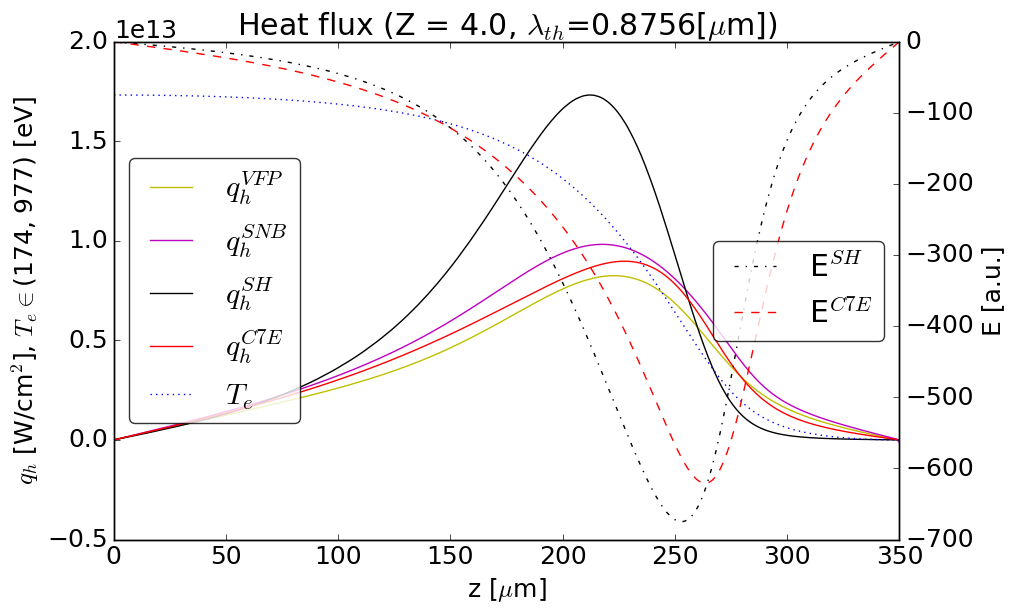
\includegraphics[width=1.0\textwidth]{../VFPdata/C7_heatflux_12ps.png} \\ 
      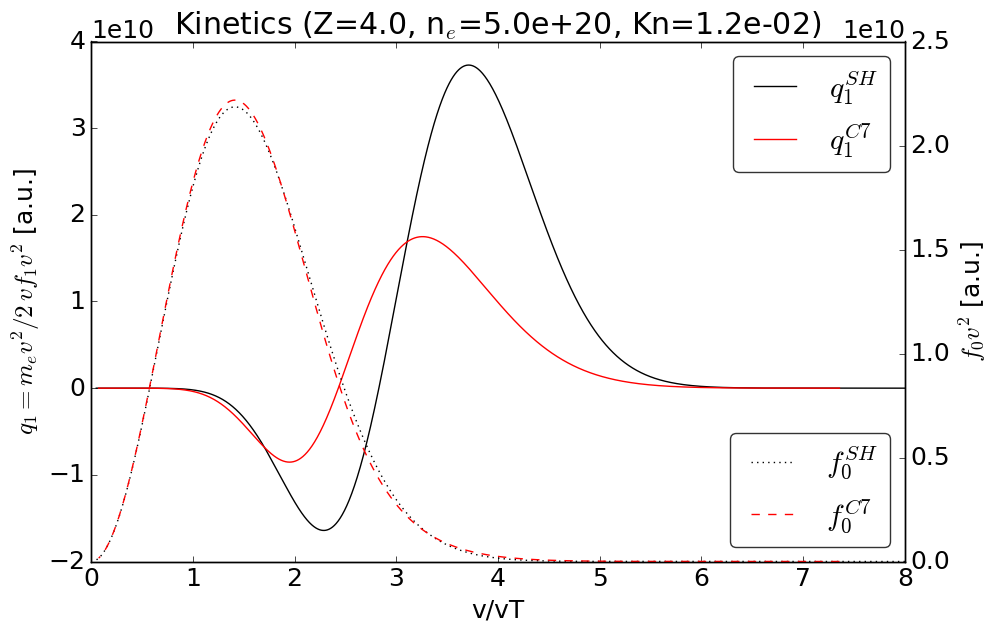
\includegraphics[width=1.0\textwidth]{../VFPdata/C7_kinetics_12ps.png}
    \end{tabular}
  \caption{
  Philippe's preferred test $\Zbar = 4$ at 12 ps.  
  }
  \end{center}
  \label{fig:Philippe_VFP_12ps}
\end{figure}

\begin{figure}[tbh]
  \begin{center}
    \begin{tabular}{c}
      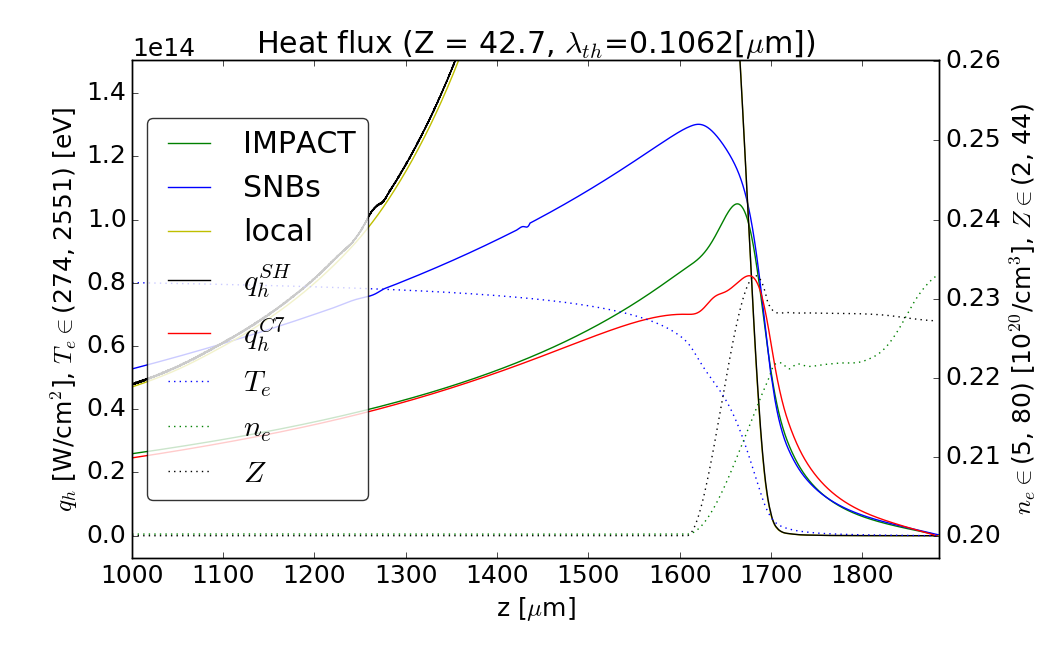
\includegraphics[width=1.0\textwidth]{../VFPdata/GD_Hohlraum/fluxes_10ps.png} \\
      %\includegraphics[width=1.0\textwidth]{../VFPdata/GD_Hohlraum/diffusion_fluxes_10ps.png} 
      %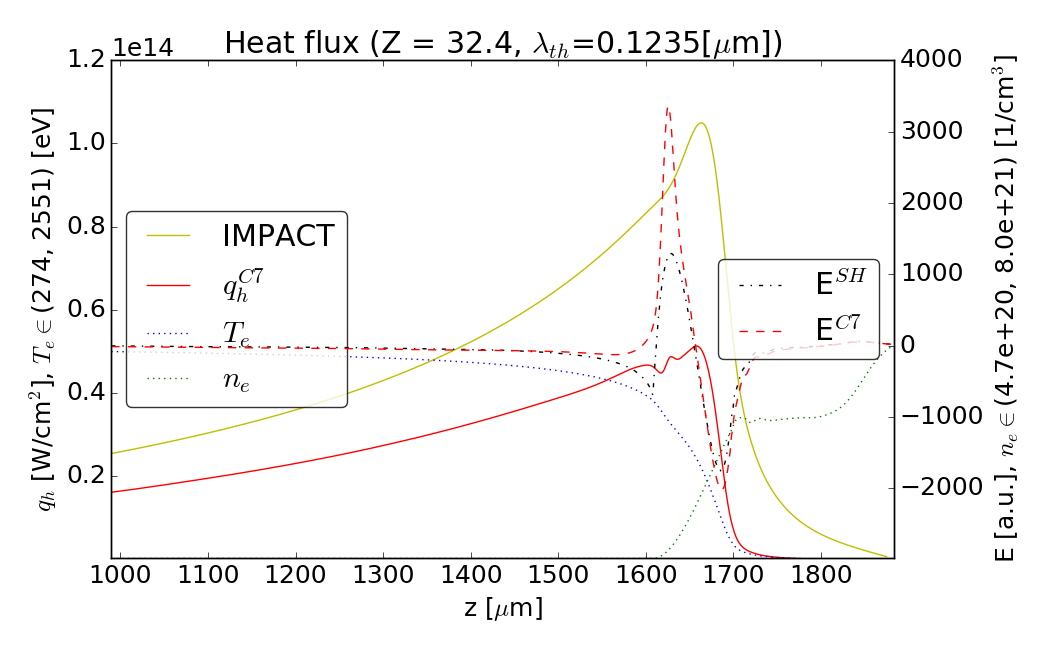
\includegraphics[width=1.0\textwidth]{../VFPdata/GD_Hohlraum/fluxes_Efield_10ps.png} \\ 
      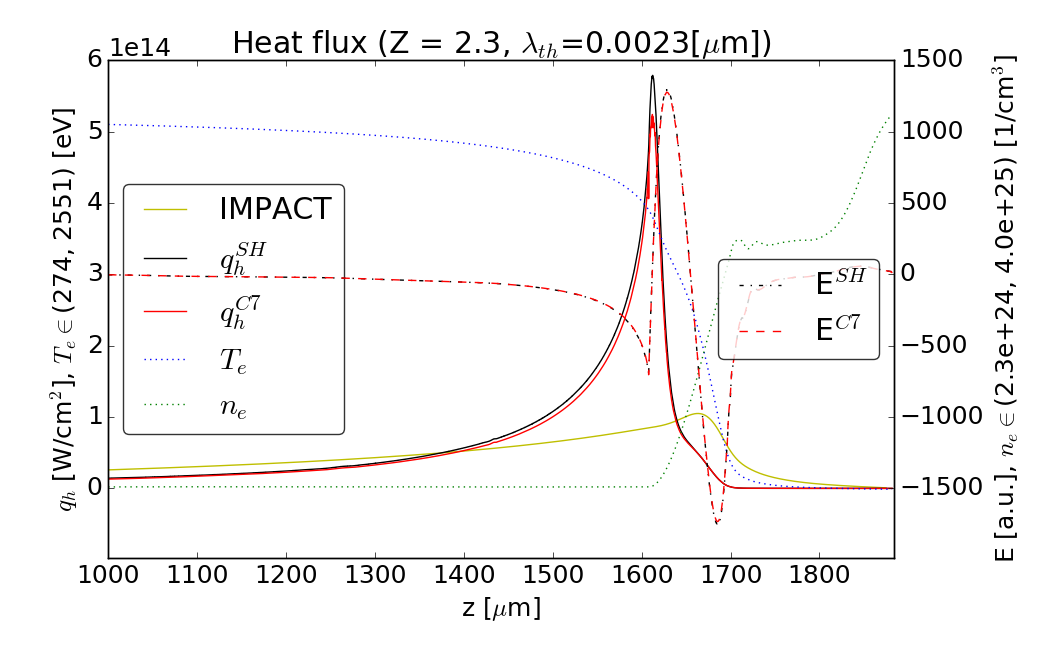
\includegraphics[width=1.0\textwidth]{../VFPdata/GD_Hohlraum/diffusion_fluxes_Efield_10ps.png} 
    \end{tabular}
  \caption{
  }
  \end{center}
  \label{fig:Gd_VFP_10ps_heatflux}
\end{figure}

\begin{figure}[tbh]
  \begin{center}
    \begin{tabular}{c}
       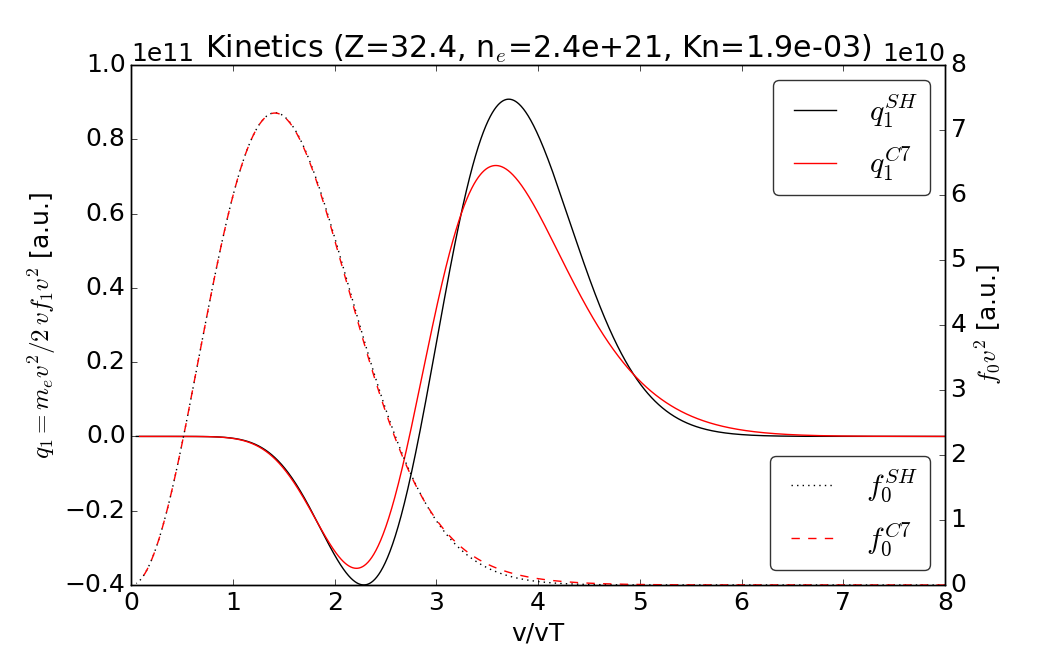
\includegraphics[width=1.0\textwidth]{../VFPdata/GD_Hohlraum/kinetics_10ps_xpointmax.png} \\ 
      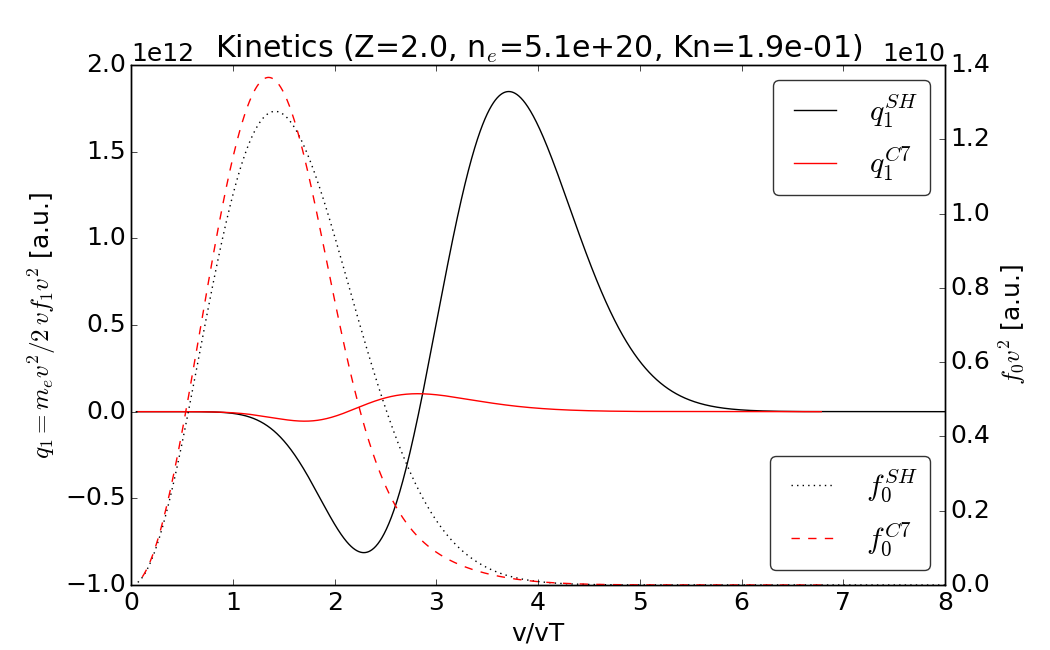
\includegraphics[width=1.0\textwidth]{../VFPdata/GD_Hohlraum/kinetics_10ps_xpoint_1605microns.png}
    \end{tabular}
  \caption{
  Kinetics profiles for max(flux) point and 1605 microns point for the case of 10ps VFP temperature profile, ne and Z Hydra profiles. 
  }
  \end{center}
  \label{fig:Gd_VFP_10ps_kinetics}
\end{figure}

\begin{figure}[tbh]
  \begin{center}
    \begin{tabular}{c}
      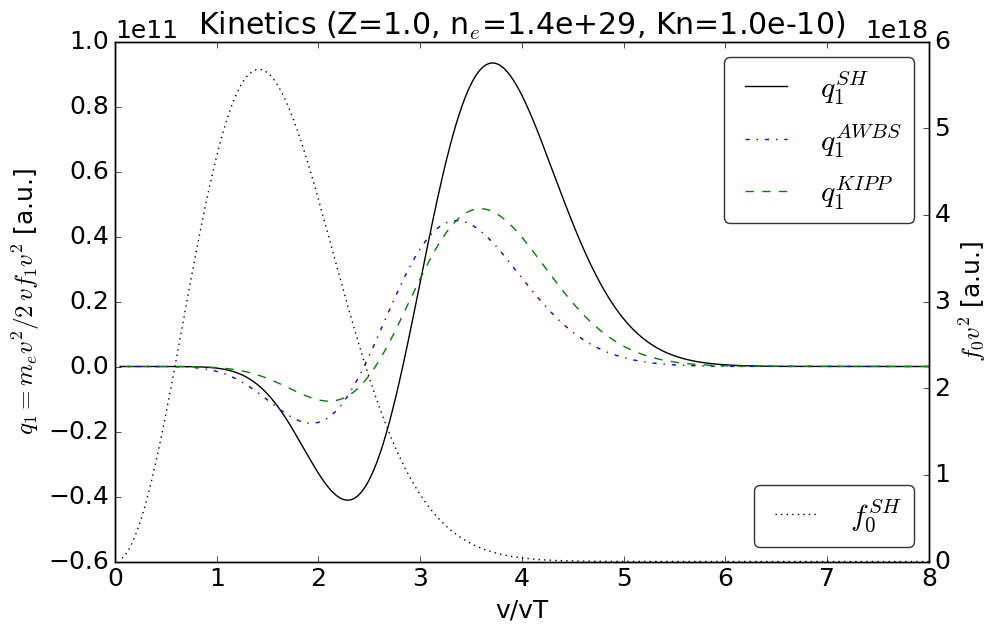
\includegraphics[width=1.0\textwidth]{../VFPdata/KIPP_q_kinetics.png} \\
      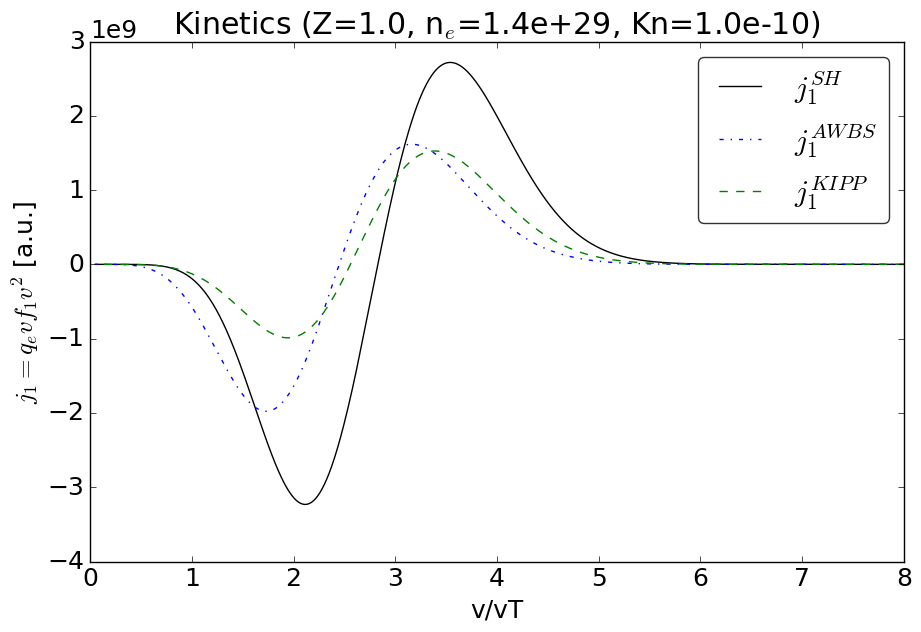
\includegraphics[width=1.0\textwidth]{../VFPdata/KIPP_j_kinetics.png}
    \end{tabular}
  \caption{KIPP (by Johnathan) vs AWBS using 
  $\mfpei^* = \frac{\Zbar + 0.24}{\Zbar + 4.2}\mfpei, \Zbar=1, 
  \vth = \sqrt{\frac{\kB T_e}{\me}}$ 
  $f_1^{SH} = -\mfpei^*(v) \left(\frac{v^2}{2 \vth^2} - 4\right) 
  \frac{\vn\cdot\nabla T_e}{T_e} \fM,\quad 
  f_1^{KIPP} = -\mfpei^*(v) \left(\frac{3}{16}\frac{v^2}{\vth^2} - 1 
  - \frac{3}{2}\frac{\vth^2}{v^2} \right) 
  \frac{\vn\cdot\nabla T_e}{T_e} \fM$.
  }
  \end{center}
  \label{fig:}
\end{figure}

\begin{figure}[tbh]
  \begin{center}
    \begin{tabular}{c}
      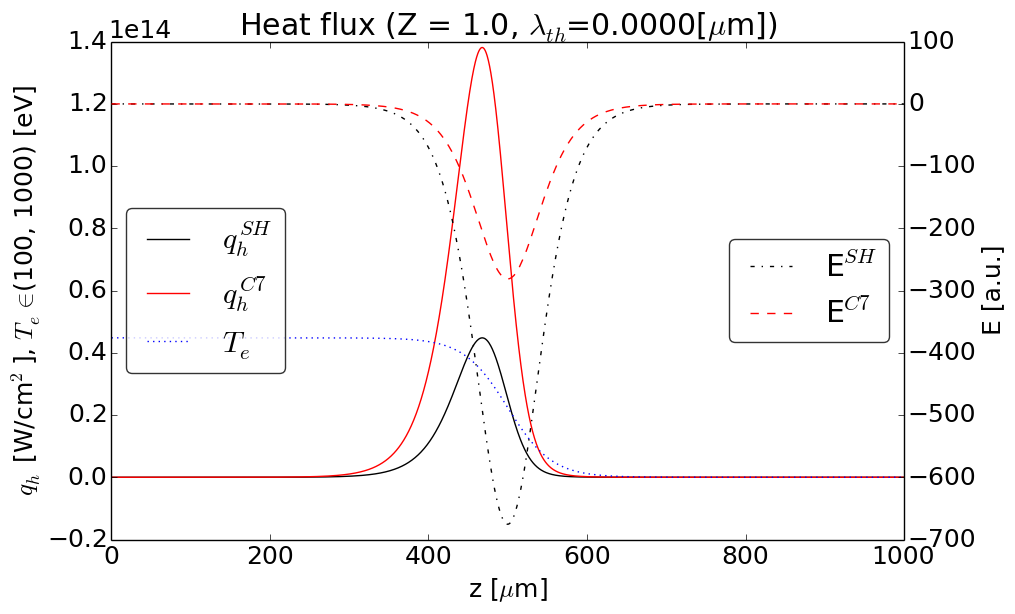
\includegraphics[width=1.0\textwidth]{../results/fe_analysis/figs/P5_diffusive_heatflux_Z1_decelerating_Ezerothiter.png} \\
      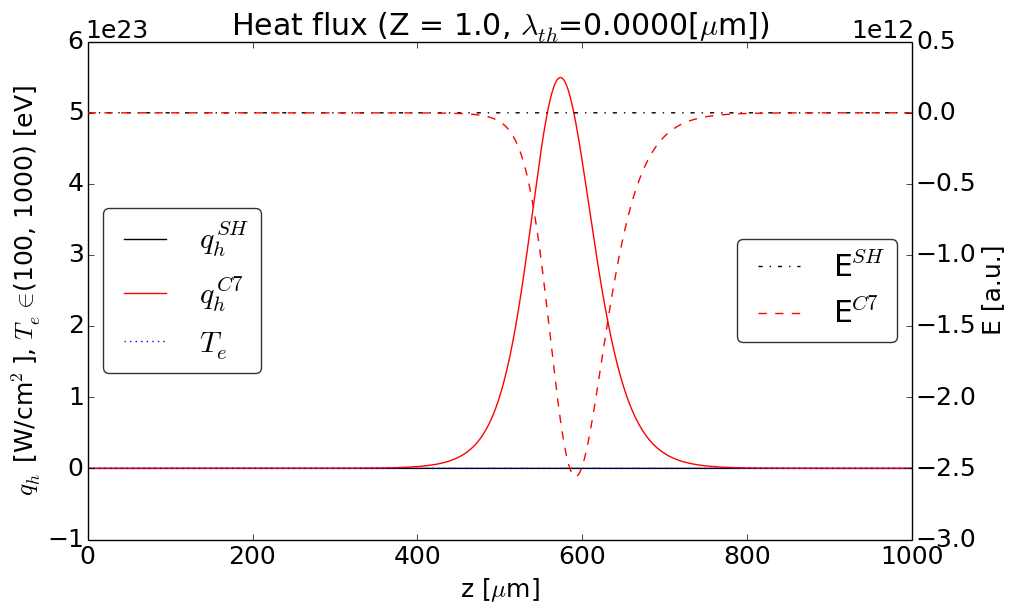
\includegraphics[width=1.0\textwidth]{../results/fe_analysis/figs/P5_diffusive_heatflux_Z1_accelerating_Ezerothiter.png}
    \end{tabular}
  \caption{
  Decelerating (top) vs. accelerating (bottom) computations. 
  Zeroth E field iteration, i.e.
  no E field effect, of the diffusion regime conditions.
  }
  \end{center}
  \label{fig:}
\end{figure}

\clearpage

%\begin{figure}[tbh]
%  \begin{center}
%    \begin{tabular}{c}
%      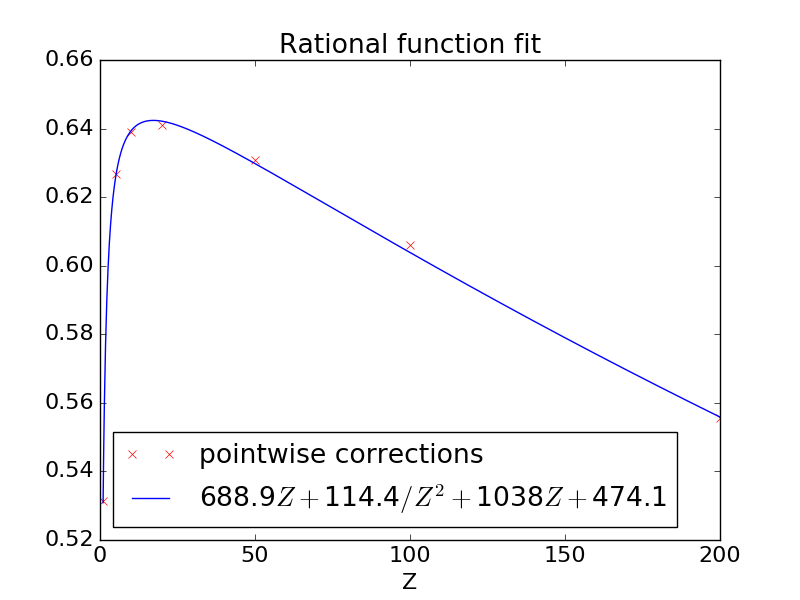
\includegraphics[width=0.55\textwidth]{../results/fe_analysis/figs/AWBScorrection_fit.png} 
%    \end{tabular}
%  \caption{
%  Analytic fit to the~Z correction 
%  ($\nue^* = \frac{688.9 \Zbar + 114.4}{\Zbar^2 + 
%  1038 \Zbar + 474.1} \nue$, where $\nue = \nuei / \Zbar$) 
%  of the~diffusion asymptotic of AWBS with respect to SH.
%  }
%  \end{center}
%  \label{fig:}
%\end{figure}

%% The Appendices part is started with the command \appendix;
%% appendix sections are then done as normal sections
%% \appendix

%% \section{}
%% \label{}

%% References
%%
%% Following citation commands can be used in the body text:
%% Usage of \cite is as follows:
%%   \cite{key}         ==>>  [#]
%%   \cite[chap. 2]{key} ==>> [#, chap. 2]
%%

%% References with bibTeX database:

\bibliographystyle{elsarticle-num}
\bibliography{NTH}

%% Authors are advised to submit their bibtex database files. They are
%% requested to list a bibtex style file in the manuscript if they do
%% not want to use elsarticle-num.bst.

%% References without bibTeX database:

% \begin{thebibliography}{00}

%% \bibitem must have the following form:
%%   \bibitem{key}...
%%

% \bibitem{}

% \end{thebibliography}


\end{document}

%%
%% End of file 
